\documentclass[xcolor=x11names,compress,professionalfonts]{beamer}

%% General packages %%%%%%%%%%%%%%%%%%%%%%%%%%%%%%%%%%
\usepackage[utf8]{inputenc}
\usepackage{graphicx}
\usepackage{tikz}
\tikzset{% change default arrow tips
    >=latex
}
\usepackage{ifthen}

\usepackage{nicefrac}

\usepackage{color}
\usepackage[english, french]{babel} %français
\usepackage{amsmath, amssymb, amsfonts, mathtools}
%\usepackage{makeidx}
%\usepackage{graphicx}
%\usepackage{braket} %quantum mechanics
%\usepackage[usenames,dvipsnames]{xcolor} % colors for text
%\usepackage[absolute]{textpos} % to place elements in the page
%\usepackage{tikz} % drawing in LaTeX
%\usetikzlibrary{positioning}
\usepackage{ dsfont } % hollow letters
%% compile child documents using this preamble
%\usepackage{subfiles}
%% compile child files with separate preambles, and include them in the document
%\usepackage{standalone}
%% subfigure
%\usepackage{subcaption}
%% include pdf pages in the document
%\usepackage{pdfpages}
%% hyperlinks
%\usepackage[colorlinks=true, linkcolor=black, citecolor=black]{hyperref}
%% BODY command inside new environments
%\usepackage{environ}
%% lots of nice custom commands for physicists
\usepackage{physics}
\usepackage{forloop}
%% if structures
%\usepackage{xifthen}
%% include figures in text blocs
%\usepackage{wrapfig}
%% algorithms
%\usepackage{algorithmic, algorithm}
%\usepackage{nicefrac}

%%%%%%%%%%%%%%%%%%%%%%%%%%%%%%%%%%%%%%%%%%%%%%%%%%%%%%

\makeatletter
\setbeamertemplate{footline}
{
    \leavevmode%
    \hbox{%
        \begin{beamercolorbox}[wd=.333333\paperwidth,ht=2.25ex,dp=1ex,center]{author in head/foot}%
            \usebeamerfont{author in head/foot}\insertshortauthor
        \end{beamercolorbox}%
                \begin{beamercolorbox}[wd=.333333\paperwidth,ht=2.25ex,dp=1ex,center]{title in head/foot}%
            \usebeamerfont{title in head/foot}\insertshorttitle
        \end{beamercolorbox}%
        \begin{beamercolorbox}[wd=.333333\paperwidth,ht=2.25ex,dp=1ex,right]{date in head/foot}%
            \usebeamerfont{date in head/foot}\insertshortdate{}\hspace*{2em}
            \insertframenumber{} / \inserttotalframenumber\hspace*{2ex} 
        \end{beamercolorbox}}%
        \vskip0pt%
    }
    \makeatother


%% Beamer Layout %%%%%%%%%%%%%%%%%%%%%%%%%%%%%%%%%%
\useoutertheme[subsection=false,shadow]{miniframes}
\useinnertheme{rectangles}

\setbeamertemplate{navigation symbols}{}%remove navigation symbols

\author{Nicolas Macé}

\newcommand{\btVFill}{\vskip0pt plus 1filll}%place an element at the bottom of the page

\usepackage{libertine}
\usepackage[T1]{fontenc}

\setbeamerfont{title like}{shape=\scshape}
\setbeamerfont{frametitle}{shape=\scshape}

\setbeamercolor*{lower separation line head}{bg=DeepSkyBlue4} 
\setbeamercolor*{normal text}{fg=black,bg=white} 
\setbeamercolor*{alerted text}{fg=red} 
\setbeamercolor*{example text}{fg=black} 
\setbeamercolor*{structure}{fg=black} 
 
\setbeamercolor*{palette tertiary}{fg=black,bg=black!10} 
\setbeamercolor*{palette quaternary}{fg=black,bg=black!10} 

\renewcommand{\(}{\begin{columns}}
\renewcommand{\)}{\end{columns}}
\newcommand{\<}[1]{\begin{column}{#1}}
\renewcommand{\>}{\end{column}}

% custom commands and definitions
%------------------ General setup ------------------%
\definecolor{darkblue}{rgb}{0.0,0.0,0.4}
\hypersetup
{
bookmarksopen=true,
pdftitle=Nicolas Macé - Electronic properties of quasicrytals,
pdfauthor=Nicolas Macé, 
pdfsubject=Electronic properties of quasicrytals, %subject of the document
%pdftoolbar=false, % toolbar hidden
pdfmenubar=true, %menubar shown
pdfhighlight=/O, %effect of clicking on a link
colorlinks=true, %couleurs sur les liens hypertextes
pdfpagemode=None, %aucun mode de page
pdfpagelayout=SinglePage, %ouverture en simple page
pdffitwindow=true, %pages ouvertes entierement dans toute la fenetre
linkcolor=darkblue, %couleur des liens hypertextes internes
citecolor=RoyalBlue, %couleur des liens pour les citations
urlcolor=darkblue %couleur des liens pour les url
}

%---------------- Commands ---------------------------%

%%%%%%%%%%%%%% TYPOGRAPHY %%%%%%%%%%%%%%%%%%%%%%%%%%%%%

% id est
\newcommand{\ie}{i.e.}
% eg
\newcommand{\eg}{e.g.}

%%%%%%%%%%%%%% MISC %%%%%%%%%%%%%%%%%%%%%%%%%%%%%%%%%%%%%

% et al
\newcommand{\etal}{\textit{et~al.}\xspace}
% vector notation
\renewcommand{\vec}[1]{\mathbf{#1}}
% the equal sign I use to define something
\newcommand{\define}{\ensuremath{ \overset{\text{def}}{=} }}
% card sine
\DeclareMathOperator{\sinc}{sinc}
% differential element
\renewcommand{\d}[1]{\mathrm{d}#1}
% similar symbol with a limit underneath
\newcommand{\simlim}[1]{\ensuremath{ \underset{#1}{\sim} }}
% alias for omega
\newcommand{\om}{\ensuremath{\omega}}
% local part of the KK wavefunction
\DeclareMathOperator{\loc}{C}
% idos
\newcommand{\idos}{\ensuremath{\text{idos}}}
% hermitian conjugate
\newcommand{\hc}{\ensuremath{\text{H.c}}}
% region on the tiling
\newcommand{\reg}{\ensuremath{\mathcal{R}}}
% generating function of the height stat
\newcommand{\gen}{\ensuremath{Z}}
% volume of a region
\newcommand{\vol}{\ensuremath{\text{Vol}}}
% Ammann-Beenker alias
\newcommand{\AB}{Ammann-Beenker}
% SKK alias
\newcommand{\SKK}{SKK}
% sim symbol with a limit underneath
\newcommand{\simop}[1]{\ensuremath{\underset{#1}{\sim}}}

% differential element
\renewcommand{\d}[1]{\mathrm{d}#1}

\newcommand{\lb}{\ensuremath{\overline{\lambda}}}
\newcommand{\zb}{\ensuremath{\overline{z}}}
% wavefunction dimensions
\newcommand{\wf}{\ensuremath{d^\psi}}
% averaged wavefunction dimensions
\newcommand{\avwf}{\ensuremath{\overline{D^\psi}}}
% local spectral dimensions
\newcommand{\locspec}{\ensuremath{D^\mu}}
% averaged local spectral dimensions
\newcommand{\avspec}{\ensuremath{D^\mu}}
% bold g letter in math mode
\newcommand{\gv}{\ensuremath{\mathbf{g}}}

% log derivative of the wavefunction
\newcommand{\dlogpsi}{\ensuremath{\d \log \psi}}
% average potential
\newcommand{\meanv}{\ensuremath{\langle V \rangle}}
% ceiling function
\DeclarePairedDelimiter{\ceil}{\lceil}{\rceil}
% floor function
\DeclarePairedDelimiter{\floor}{\lfloor}{\rfloor}
% irrational number
\newcommand{\irr}{\ensuremath{\alpha}}
% cut-and-project
\renewcommand{\cp}{C\&P}
% set of the integers
\newcommand{\zahl}{\ensuremath{\mathds{Z}}}
% fractional part function
\DeclarePairedDelimiter{\fpart}{\{}{\}}
% normalized perp position
\newcommand{\nperp}[2]%
	{%
		\ifthenelse{\isempty{#1}}{\ensuremath{\widetilde{x}_\perp}}{\ensuremath{\widetilde{x}_\perp(#1,#2)}}%
	}
% average with angled brackets
\DeclarePairedDelimiter{\avg}{\langle}{\rangle}
% sturmian fucntion (generate a sturmian sequence)
\newcommand{\sturm}[2]{\ensuremath{S_{#1}\left(#2\right)}}
% Heaviside function
\DeclareMathOperator{\heaviside}{Y}
% support of the multifractal spectrum
\newcommand{\supp}{\ensuremath{\Delta_f}}
% variational groundstate
\newcommand{\psivar}{\ensuremath{\psi_\text{var}}}
% preexponential factor for the variational groundstate
\newcommand{\locvar}{\ensuremath{C_\text{var}}}

%%%%%%%%%%%%%%%%% COMMENTS %%%%%%%%%%%%%%%%%%%%%%%%%%%
\newcommand{\nico}[1]{\textcolor{BrickRed}{#1}}
\newcommand{\anu}[1]{\textcolor{NavyBlue}{#1}}
\newcommand{\fred}[1]{\textcolor{OliveGreen}{#1}}

%%%%%%%%%%%%%%%% QUANTUM MECHANICS %%%%%%%%%%%%%%%%%
% energy
\newcommand{\en}{\ensuremath{\varepsilon}}
% Operator
\renewcommand{\op}[1]{\hat{#1}}
% density of states
\DeclareMathOperator{\dos}{\rho}

%%%%%%%%%%%%%%%% ALPHABETS AND WORDS %%%%%%%%%%%
% the A letter
\newcommand{\A}{\ensuremath{\text{A}}}
% the B letter
\newcommand{\B}{\ensuremath{\text{B}}}
% any sequence of letters
\newcommand{\lett}[1]{\ensuremath{\text{#1}}}
% letter couting function: #1 is the word we count in, #2 is the sequence of letters counted
\newcommand{\nb}[2]{\ensuremath{|#1|_{#2}}}
% substitution
\DeclareMathOperator{\sub}{S}
% word (infinite)
\newcommand{\word}{\ensuremath{w}}
% word complexity
\newcommand{\cmplx}[2]%
	{%
		\ifthenelse{\isempty{#1}}{\ensuremath{\Omega}}{\ensuremath{\Omega(#1,#2)}}%
	}

%%%%%%%%%%%%%%% PERIODIC CRYSTALS %%%%%%%%%%%%%%
\newcommand{\kvec}{\ensuremath{\mathbf{k}}}

%%%%%%%%%%%%%%% MULTIFRACTAL ANALYSIS %%%%%%%%%%
\newcommand{\bc}{box-counting}
% mass (or probability measure) defining a fractal set
\DeclareMathOperator{\mass}{\mu}
% q weight
\DeclareMathOperator{\qweight}{\text{M}}
% partition into a set of boxes
\DeclareMathOperator{\boxset}{\mathcal{B}}
% pointwise Hölder exponent
\DeclareMathOperator{\hold}{\alpha}



\begin{document}

\begin{frame}
\title{Thermalization and localization in one-dimensional quantum systems}

\author{Nicolas Macé}

\date{Janurary 30, 2019}

\titlepage

\btVFill
\begin{columns}
\begin{column}{2cm}
~\\
~\\
~\\
~\\
\raggedright
\includegraphics[scale=.15]{img/title/logo-ups.png}
\end{column}
\begin{column}{6cm}
\centering
\includegraphics[width=.8\textwidth]{img/title/cover.png}
\end{column}
\begin{column}{2cm}
~\\
~\\
~\\
~\\
\raggedleft
\includegraphics[scale=.15]{img/title/LPT-LOGO_RVB.jpg}
\end{column}
\end{columns}
\end{frame}

\section{Introduction}
%Each section needs a subsection for the small points on top to show up
\subsection{Dummy}

\begin{frame}{Quasicrystals}
\(
	\<{6cm}
		\centering
		\includegraphics[scale=0.28]{img/1_intro/homgzn.png}
		
		\ss{3D HoMgZn quasicrystalline sample} \ss{(\url{doi:10.1038/nmat1244})}
	\>
	\<{6cm}
		\centering
		\includegraphics[scale=0.22]{img/1_intro/wasio.jpg}
		
		\ss{A 2D molecular quasicrystal} \ss{(\url{doi:10.1038/nature12993})}
	\>
\)

\begin{itemize}
	\item \ss{Fractal dimensions of wave functions and local spectral measures on the Fibonacci chain}\\\emph{Macé, Jagannathan, Piéchon, PRB 93 (20), 2016}
	\item \ss{Critical eigenstates and their properties in one-and two-dimensional quasicrystals}\\
	\emph{Macé, Jagannathan, Kalugin, Mosseri, Piéchon, PRB 96 (4), 2017}
\end{itemize}
\end{frame}

\begin{frame}{A quasiperiodic puzzle [Bédaride \etal{} 12]}

\centering
\includegraphics[width=.4\textwidth]{img/1_intro/tiles_euro.pdf}

Pay the squares, get the rhombuses for free!

\(
\<{6cm}
\centering
\includegraphics[width=.8\textwidth]{img/1_intro/forbidden.pdf}

Forbidden configuration.
\>

\<{6cm}
\centering

\includegraphics[width=1.\textwidth]{img/1_intro/ammann.pdf}

Patch of the Ammann-Beenker tiling.
\>
\)
\end{frame}

\begin{frame}{Periodic, quasiperiodic and random}
\only<1>{
A random tiling:

\centering
\includegraphics[width=.4\textwidth]{img/1_intro/random00.pdf}

}

\only<2>{
Two copies of the tiling:

\centering
\includegraphics[width=.75\textwidth]{img/1_intro/random01.pdf}

}

\only<3>{
\centering
\includegraphics[width=.6\textwidth]{img/1_intro/random.pdf}

$\to$ no overlap $\to$ no order}

\centering
\only<4>{
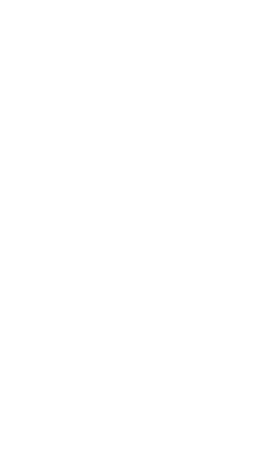
\includegraphics[width=.6\textwidth]{img/1_intro/periodic.pdf}

Perfect long range order: periodic}

\only<5>{

\includegraphics[width=.6\textwidth]{img/1_intro/quasiperiodic.pdf}

Long range order: quasiperiodic 

\flushleft{(see Chap.\ 2 of [Grimm, Baake 13])}
}

\end{frame}

%\begin{frame}{From tiles to atoms}
%Place atoms at the vertices of the tiling:
%
%{\centering
%\includegraphics[width=.6\textwidth]{img/1_intro/AB_tiling_and_plot.pdf}
%
%}
%
%$\rightarrow$ can atoms arrange in such a quasiperiodic fashion?
%\end{frame}

\begin{frame}{Quasicrystals}
Quasicrystal $\to$ quasiperiodically arranged atoms:
\begin{itemize}
	\item \textbf{aperiodicity}
	\item \textbf{long range order} (diffraction pattern exhibits sharp peaks).
\end{itemize}
\(
	\<{6cm}
		\centering
		\includegraphics[scale=0.1]{img/1_intro/diffraction_tenfold.png}
		
		\ss{Diffraction pattern of a AlPdMn alloy} \ss{(Conradin Beeli group)}
	\>
	\<{6cm}
		\centering
		\includegraphics[scale=0.06]{img/1_intro/penrose.png}
		
		\ss{A patch of the quasiperiodic Penrose tiling,} \ss{used to model many quasicrystals.}
	\>
\)
\end{frame}

\begin{frame}{Engineered quasiperiodic structures}
\centering
\includegraphics[width=.5\textwidth]{img/1_intro/dielectric_resonators.png}

{\ss{A network of dielectric resonators [Vignolo \etal{} 14]}}

\begin{itemize}
	\item Plasmons in semiconductor stacks [Merlin \etal{} 85]
	\item Microwaves in perforated metallic films [Matsui \etal{} 07]
	\item Microwaves in dielectric resonator networks [Vignolo \etal{} 14]
	\item Light solitons [Freedman \etal{} 07]
	\item Cold atoms in laser potentials [Guidoni \etal{} 97]
	\item Polaritons in wire cavities [Tanese \etal{} 14]
\end{itemize}
\end{frame}


\begin{frame}{Fractals}
Fractal: object invariant under rescaling
\(
\<{7cm}
\centering
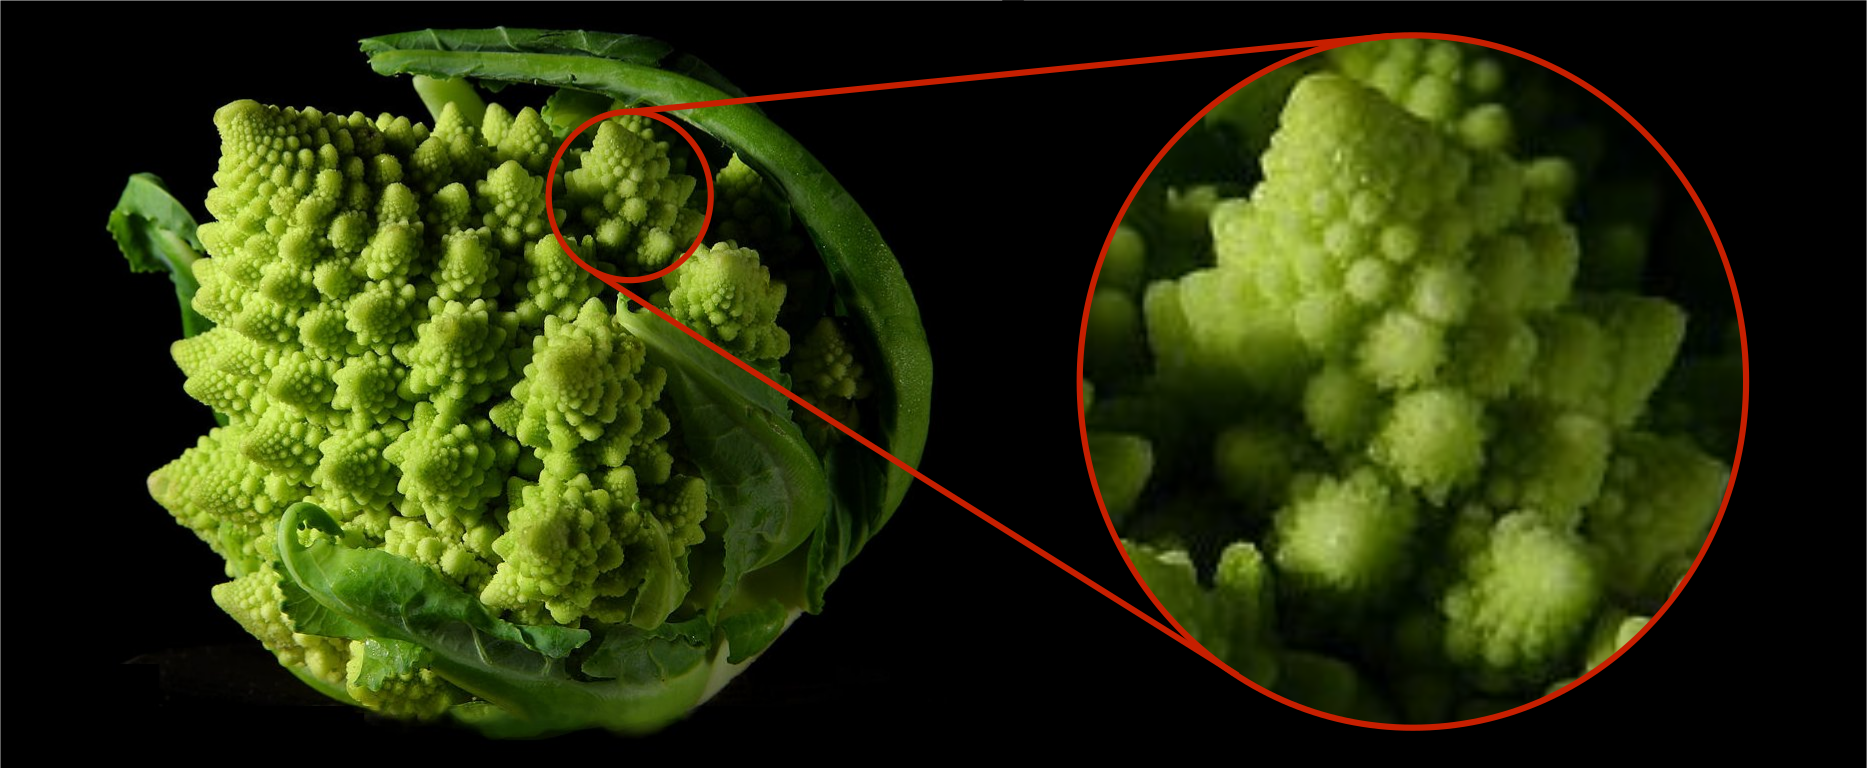
\includegraphics[width=1.\textwidth]{img/1_intro/Fractal_Broccoli.png}

{\ss Romanesco broccoli (\copyleft{} Wikimedia commons)}
\>
\<{7cm}
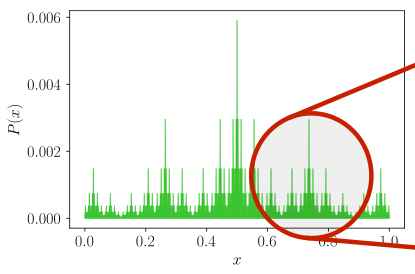
\includegraphics[width=1.\textwidth]{img/1_intro/heights.pdf}

{\ss Electronic density along a quasiperiodic chain}
\>
\)

Quasicrystals \emph{not} fractal\dots

\dots but electrons on quasicrystals $\to$ fractal behavior

\begin{beamerboxesrounded}%
        [shadow=true]%
        {Goal:}
\textbf{Link the fractal behavior of the electrons to quasiperiodicity}
\end{beamerboxesrounded}
\end{frame}
%\begin{frame}{Content}
%\tableofcontents[hideallsubsections]
%\end{frame}
\section{Introduction}
%Each section needs a subsection for the small points on top to show up
\subsection{Dummy}

\begin{frame}{Electronic properties of quasicrystals}

\end{frame}


\end{document}